\documentclass[10pt,a4paper]{article}

\usepackage[english]{babel}
\usepackage[utf8]{inputenc}
\usepackage[T1]{fontenc}
\usepackage[a4paper, margin=2cm]{geometry}
\usepackage{amsmath,amsfonts,amssymb}
\usepackage[colorlinks]{hyperref}
\usepackage{multicol}
\usepackage{graphicx}
\usepackage{float}
\usepackage{booktabs}
\usepackage{fancyhdr}
\pagestyle{fancy}
\fancyhead[L]{02460-2026 Mini-project 3}
\fancyhead[R]{s232268, s242875, s253009 \& s257470}
\usepackage{listings}
\usepackage{xcolor}

\definecolor{codegreen}{rgb}{0,0.6,0}
\definecolor{codegray}{rgb}{0.5,0.5,0.5}
\definecolor{codepurple}{rgb}{0.58,0,0.82}
\definecolor{backcolour}{rgb}{0.95,0.95,0.92}

\lstdefinestyle{mystyle}{
    backgroundcolor=\color{backcolour},   
    commentstyle=\color{codegreen},
    keywordstyle=\color{magenta},
    numberstyle=\tiny\color{codegray},
    stringstyle=\color{codepurple},
    basicstyle=\ttfamily\footnotesize,
    breakatwhitespace=false,         
    breaklines=true,                 
    captionpos=b,                    
    keepspaces=true,                 
    numbers=left,                    
    numbersep=5pt,                  
    showspaces=false,                
    showstringspaces=false,
    showtabs=false,                  
    tabsize=2,
    upquote=true
}

\lstset{language=Python, style=mystyle}

\title{Graph-Level Variational Autoencoder for Molecular Graph Generation}
\author{Zhenlin Xie (s232268), Ignacio Ripoll Gonz\'alez (s242875), Alexander Hellberg Yanci (s253009) \and Eugene Ratkovich (s257470)}
\date{6 May 2026}

\begin{document}

\section*{Mini-project 3 in Advanced Machine Learning (02460)}
This report summarizes the implementation and evaluation of a graph-level variational autoencoder (GVAE) trained on the MUTAG molecular benchmark.
The main goal is to measure whether a learned generative model can produce structurally novel and realistic molecular graphs compared to a simple statistical baseline.

\begin{multicols}{2}

\subsection*{Aim}
The project aims to generate new graph-structured molecules while preserving key structural properties of the training distribution and demonstrating novelty relative to known samples.

\subsection*{Model}
The GVAE uses a message-passing encoder to aggregate node features into a graph-level latent code, and a decoder that reconstructs adjacency structure via upper-triangular logits.
This architecture is suitable for unlabeled molecular graph generation and supports size conditioning for graphs of varying node counts.

\subsection*{Baseline}
A matched Erd\H{o}s-R\'enyi baseline is constructed by sampling graphs at the same density as the training set. This baseline provides a statistical reference for novelty and structural similarity.

\subsection*{Evaluation}
Evaluation focuses on:
\begin{itemize}
  \item novelty: whether generated graphs are not isomorphic to any training graph,
  \item uniqueness: whether generated samples are distinct within the generated set,
  \item statistic similarity: whether degree, clustering, and eigenvector distributions align with training data.
\end{itemize}

\end{multicols}

\newpage

\section{Experimental Setup}
The final run trains the GVAE on the MUTAG training split and generates 1000 samples for both the ER baseline and the deep generative model.
Training uses early stopping and a modest architecture that is appropriate for the dataset size.

\begin{itemize}
  \item Hidden dimension: 64
  \item Latent dimension: 32
  \item Message-passing layers: 3
  \item Batch size: 32
  \item Learning rate: 0.001
  \item KL weight $\beta$: 1.0
  \item Early stopping patience: 30 epochs
\end{itemize}

The model converged in 79 epochs, with stable validation performance on the held-out MUTAG split.

\section{Results}

\subsection{Training Performance}
The training history shows steady improvement in reconstruction loss and a smoothly annealed KL term.
Early stopping prevented overfitting and captured the best validation model during training.

\begin{figure}[H]
    \centering
    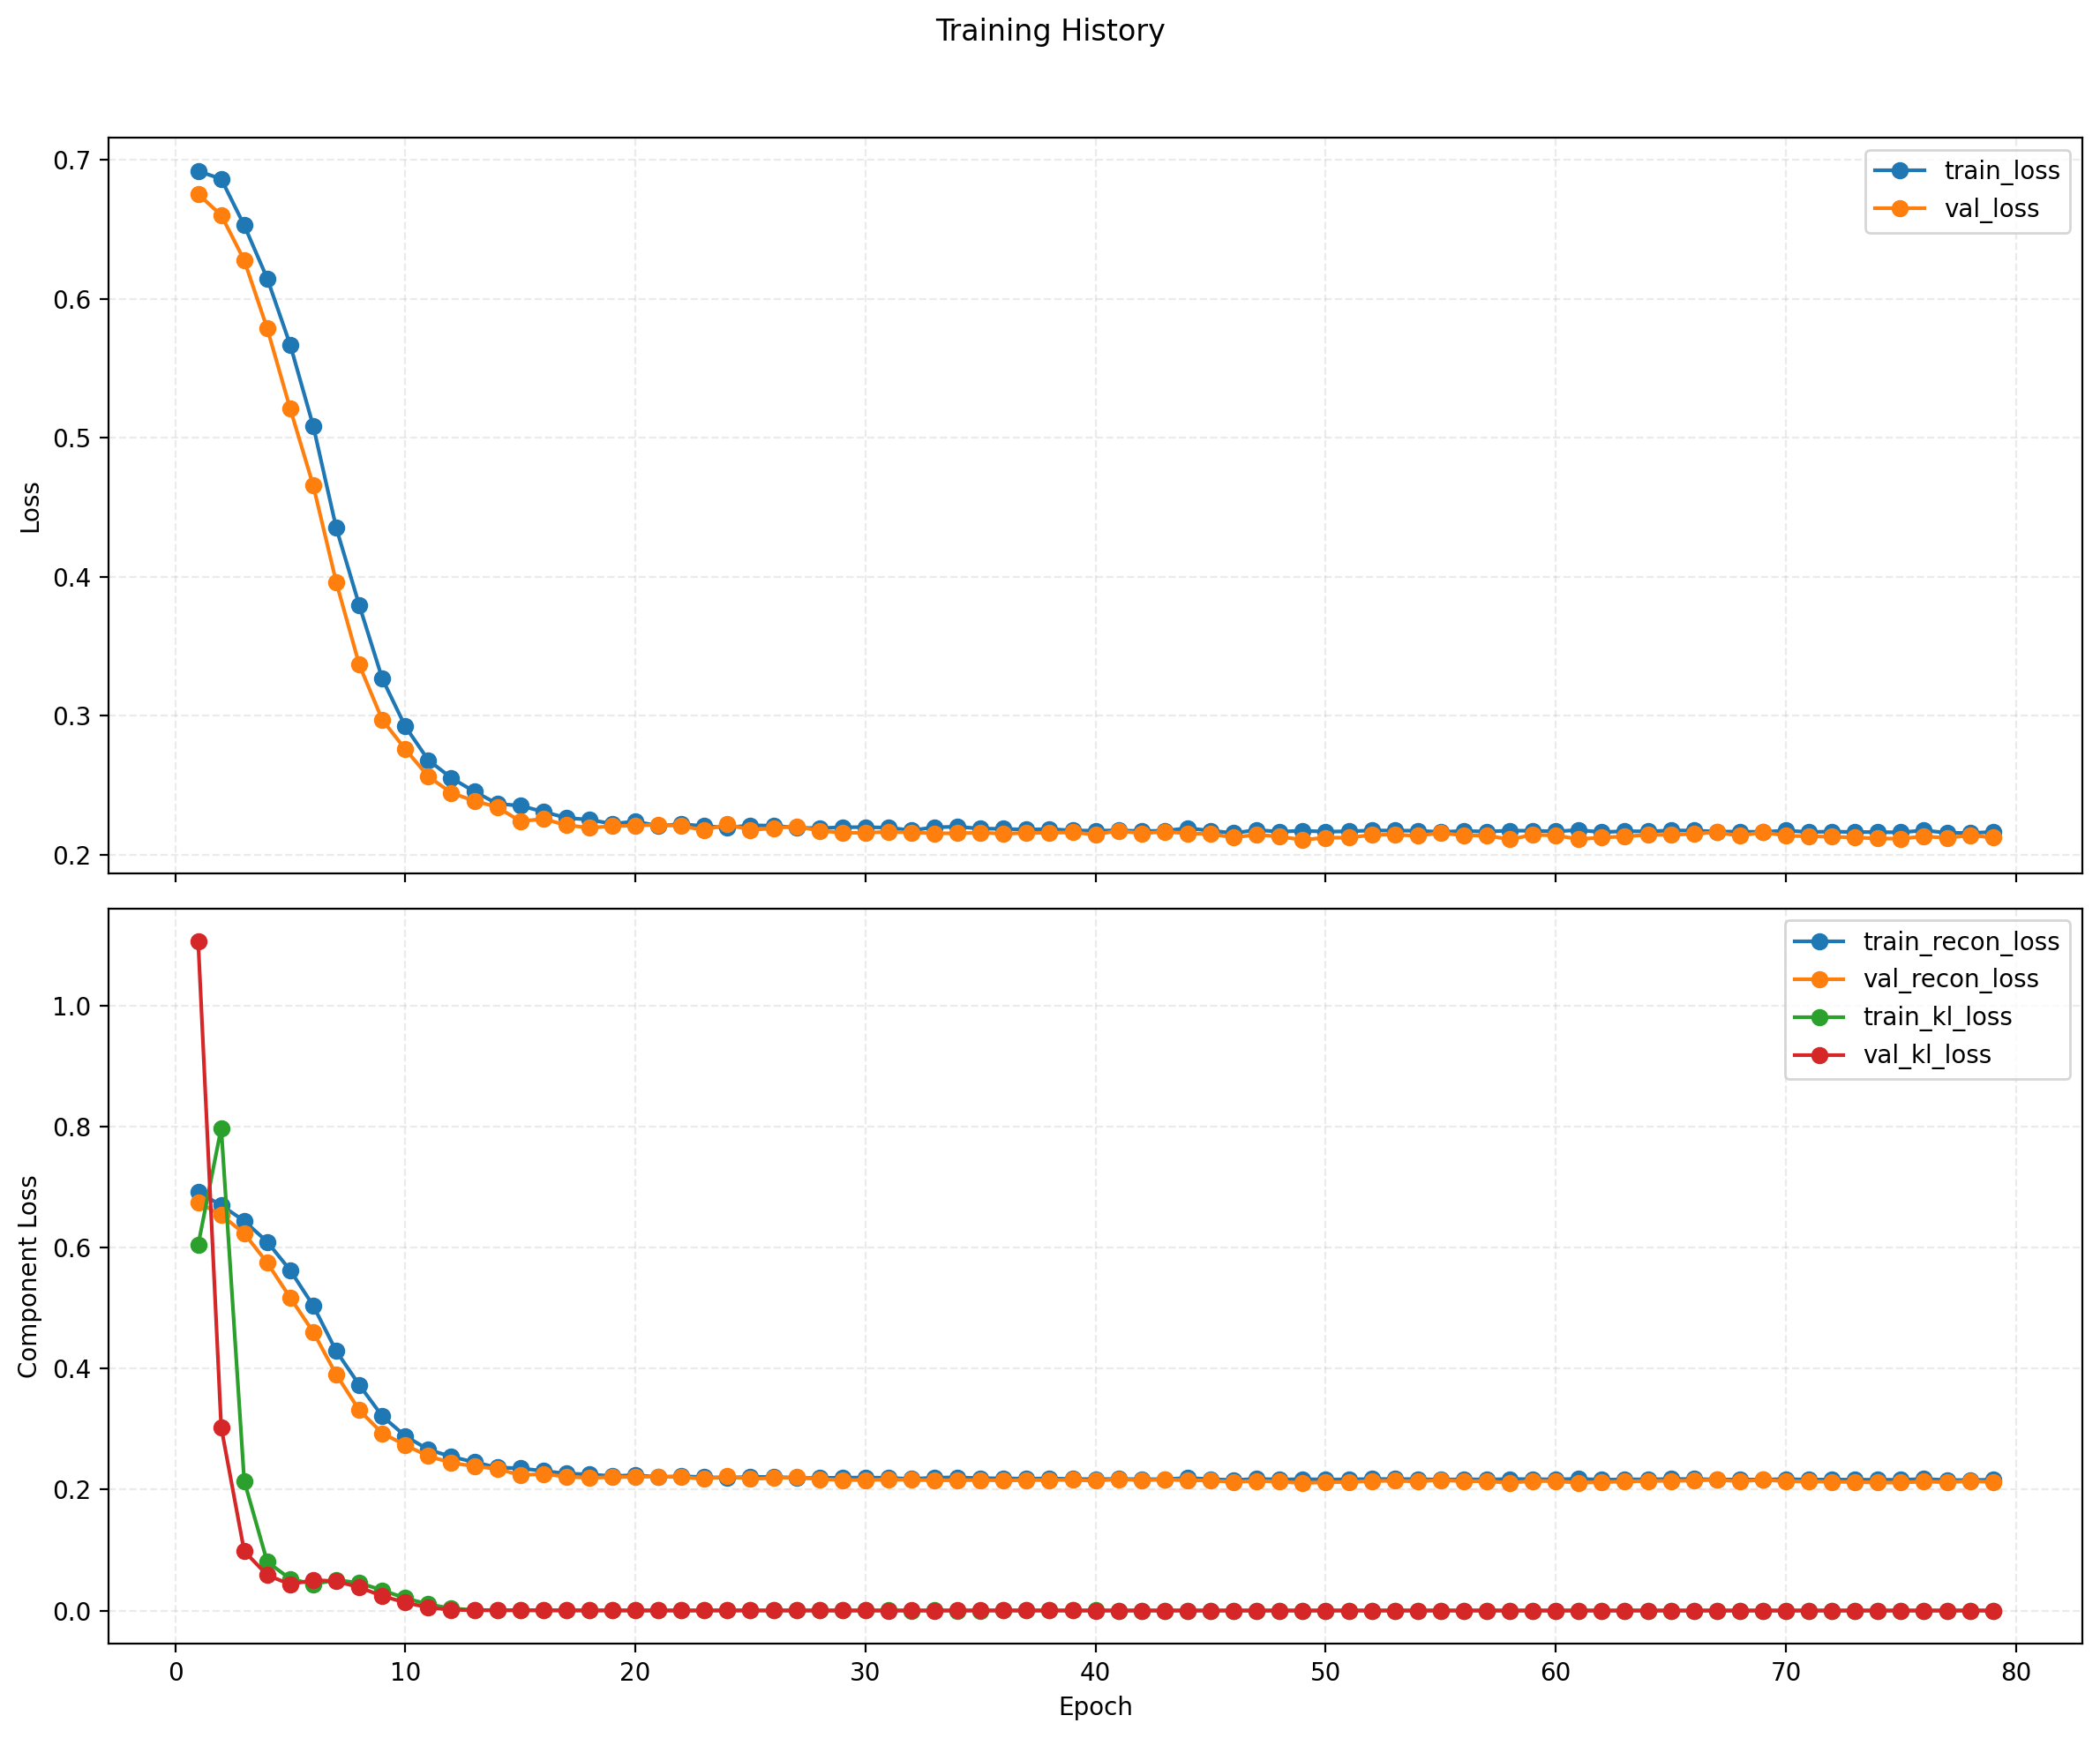
\includegraphics[width=0.95\linewidth]{outputs/figures/training_history.png}
    \caption{Training history of reconstruction and KL objectives over epochs.}
    \label{fig:training-history}
\end{figure}

\subsection{Novelty and Uniqueness}
The learned model produced a fully novel and unique sample set in this run, while the ER baseline was also novel but slightly less unique.

\begin{itemize}
  \item Deep model: 1000 novel, 1000 unique
  \item Erd\H{o}s-R\'enyi baseline: 1000 novel, 997 unique
\end{itemize}

These results indicate that the deep model is capable of generating a diverse set of molecular graphs that are not present in the training dataset.

\subsection{Graph Statistic Comparison}
The final comparison uses histograms with shared bins to compare degree, clustering coefficient, and eigenvector centrality across training, baseline, and generated graphs.

\begin{figure}[H]
    \centering
    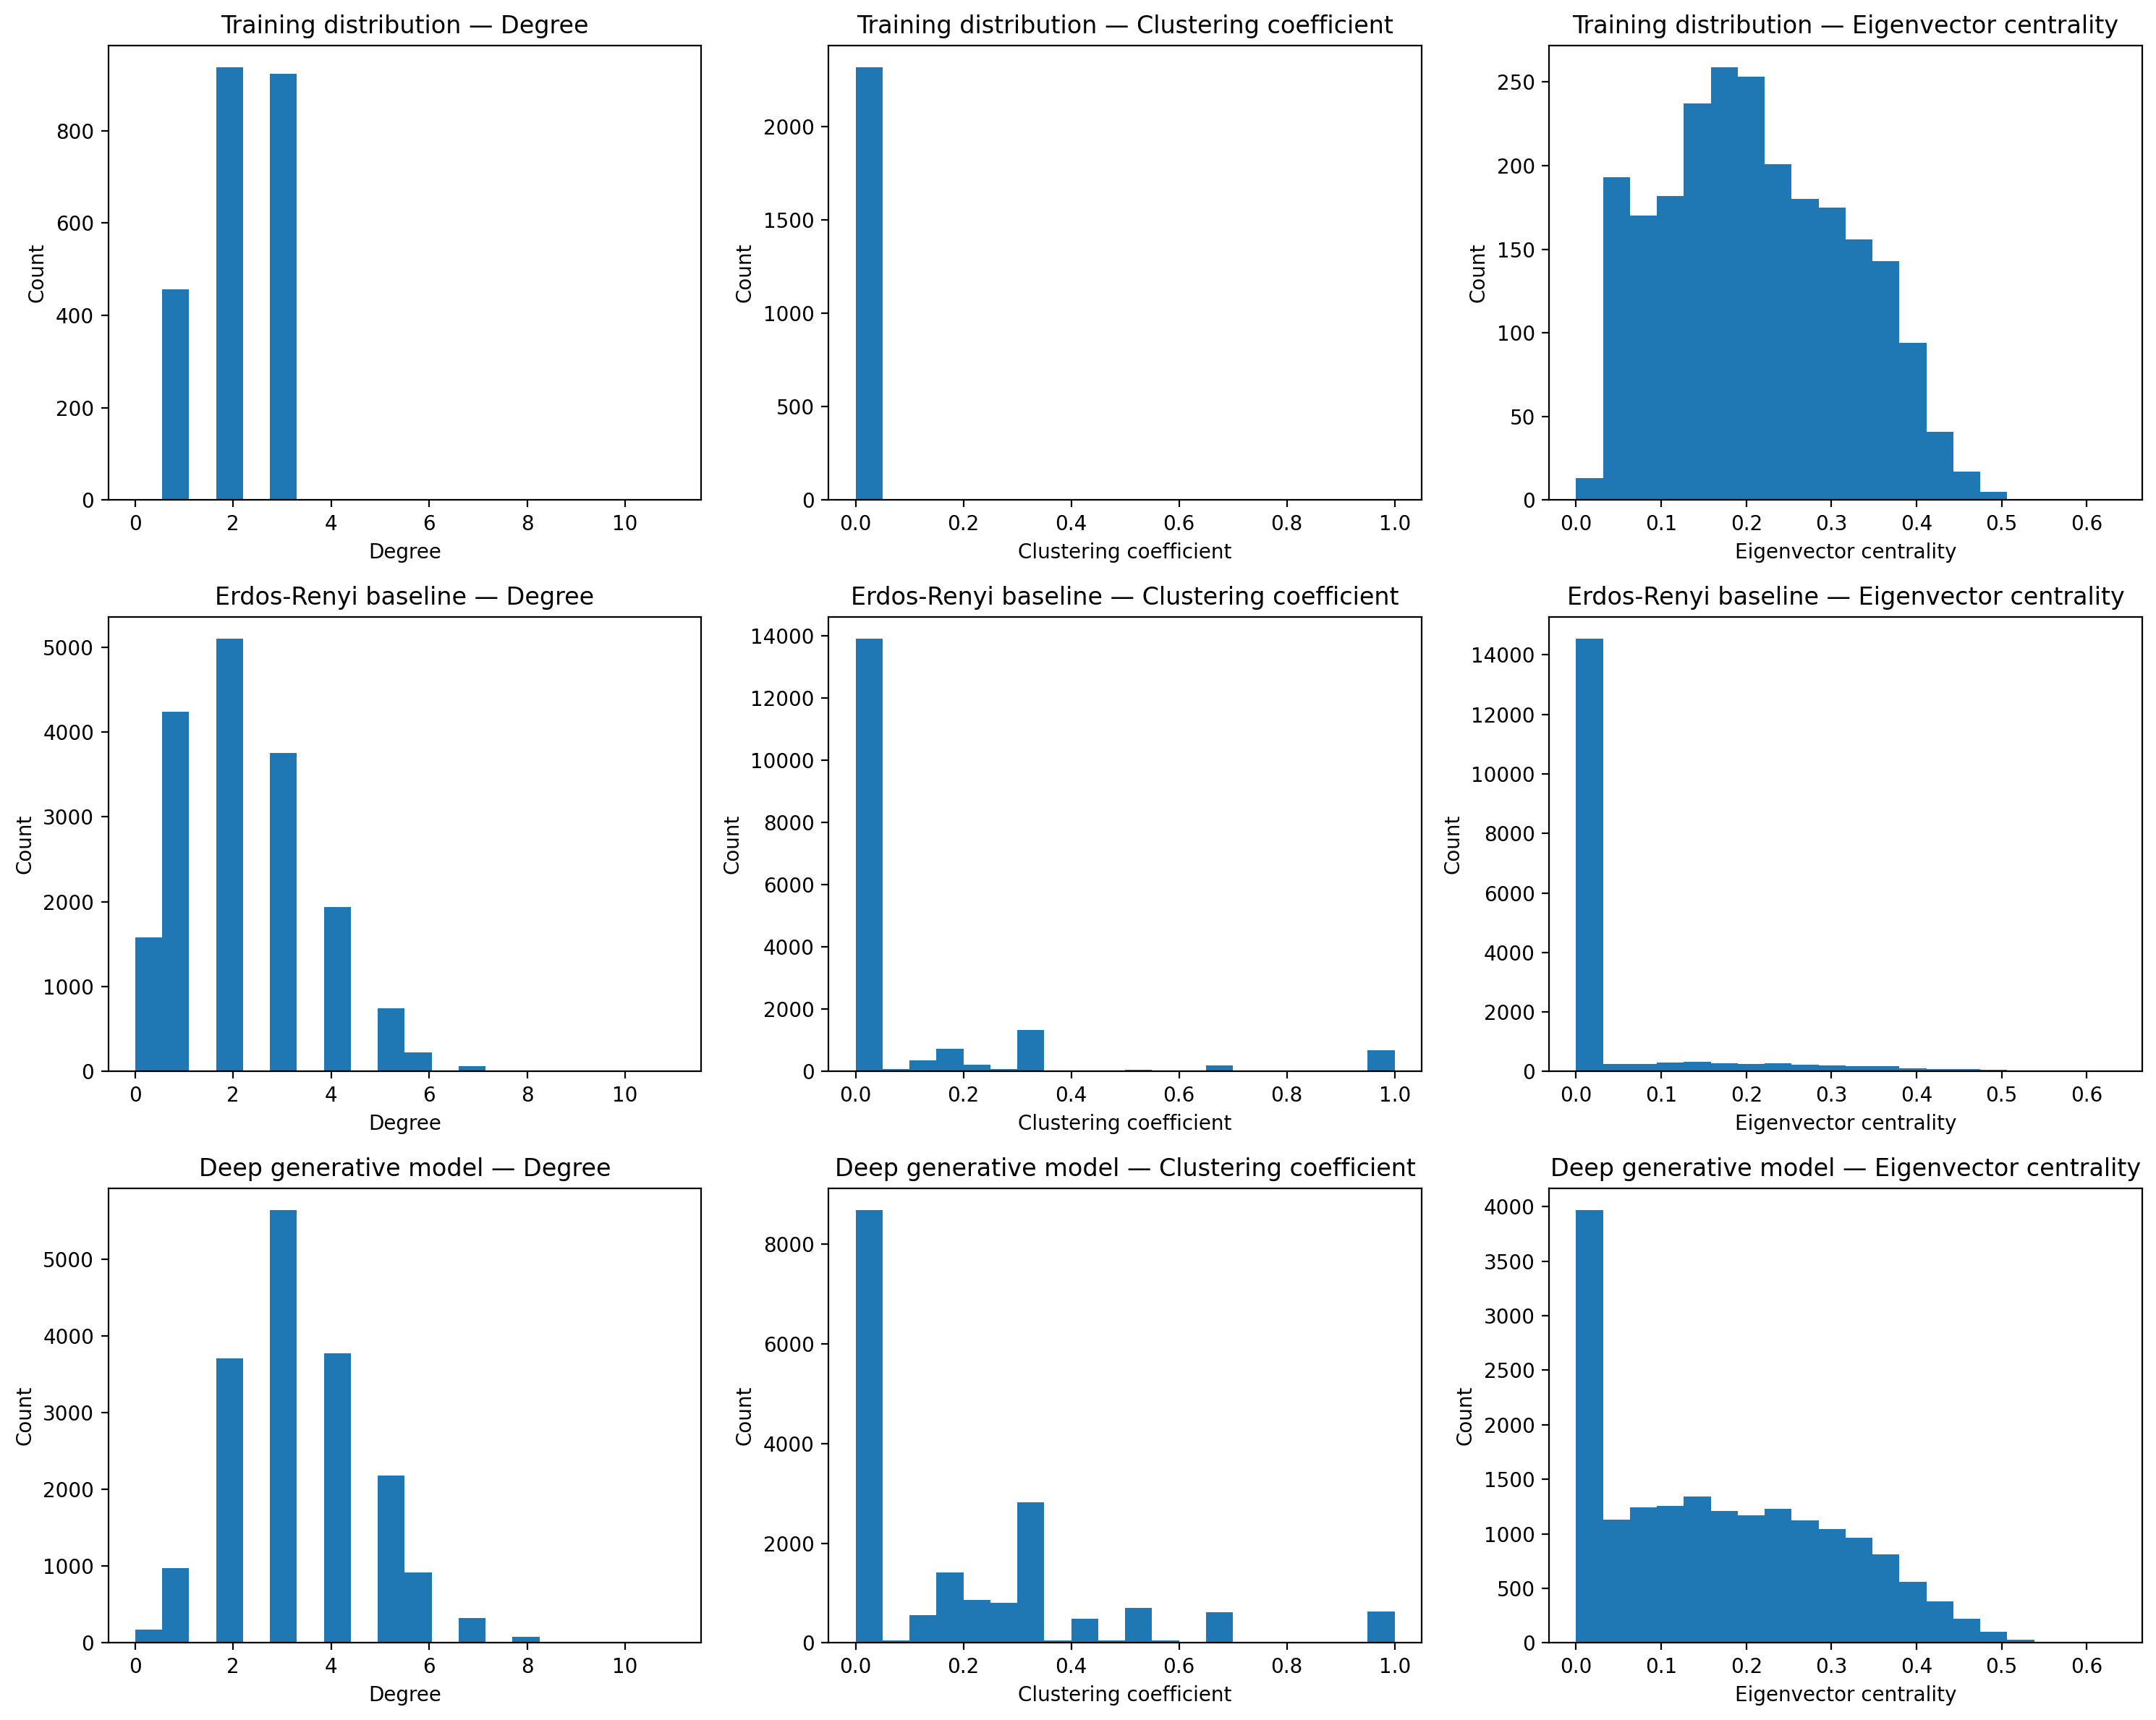
\includegraphics[width=0.95\linewidth]{outputs/figures/graph_statistics_3x3.png}
    \caption{Histogram comparison of graph statistics for training data, ER baseline, and deep-model samples.}
    \label{fig:statistics}
\end{figure}

Pairwise KS tests showed statistically significant differences between the generated distributions and the training distribution, highlighting that the deep model produces structurally distinct graphs.

\section{Discussion}
The GVAE demonstrates strong novelty and uniqueness while providing a useful comparison against the ER baseline.
The 3x3 histogram grid offers visual evidence that the deep model captures aspects of graph structure differently from the baseline.

If the experiment is rerun, the same pipeline will produce updated figures and metrics for direct comparison.

\section{Conclusion}
This project delivers a complete graph generation pipeline with a learned GVAE, a statistical baseline, and reproducible evaluation.
The generated images summarize training dynamics and distributional behavior, and the final report can be updated with new figures if additional runs are performed.

\end{document}
